\documentclass[11pt]{article}
\usepackage[margin=0.95in]{geometry}
\usepackage{booktabs}
\usepackage{tabularx}
\usepackage{xltabular} % breakable tabularx (longtable-based): avoids half-empty pages
\usepackage{array}
\usepackage{graphicx}
\usepackage{amsmath}
\usepackage{caption}
\usepackage{xcolor}
\usepackage{microtype}
\usepackage[hidelinks]{hyperref}
\captionsetup{font=small,labelfont=bf}
\setlength{\parskip}{4pt}
\setlength{\parindent}{0pt}

% Claims-table column types: Claim (flexible), Evidence (fixed), Status (fixed)
\newcolumntype{C}{>{\raggedright\arraybackslash}X}
\newcolumntype{E}{>{\raggedright\arraybackslash}p{4.7cm}}
\newcolumntype{T}{>{\raggedright\arraybackslash}p{1.9cm}}
\newenvironment{claimstable}
  {\par\footnotesize\xltabular{\textwidth}{@{}C E T@{}}
   \toprule \textbf{Claim (plain language)} & \textbf{Evidence (key numbers)} & \textbf{Status}\\ \midrule
   \endhead
   \midrule \multicolumn{3}{r@{}}{\footnotesize\emph{continued on next page}}\\
   \endfoot
   \bottomrule
   \endlastfoot}
  {\endxltabular\par\vspace{2pt}}

\title{\textbf{Consolidated Findings: Simple Policies, Information, and the Room for RL\\
in the Pharmaceutical Supply-Chain Simulator}\\
\normalsize One running document consolidating the routing study, the routing-repaired
(``understanding'') study, and the value-decomposition study (Phases 1--2,
distributor-seat test, Part C). Individual reports remain archived as the audit trail.}
\author{Aidan Hansen \quad (advisor: Prof.\ \"Ozlem Ergun)}
\date{June 11, 2026}

\begin{document}
\maketitle

\section*{How to read this document}

\textbf{The setting.} Everything in this document comes from a simulated pharmaceutical
supply chain inherited from a predecessor thesis: two manufacturers ship to two
distributors, which ship to two health centers serving patient demand (a
2$\times$2$\times$2 network). In the central experiment, one manufacturer loses 95\% of
its production capacity for 48 of the episode's 300 periods. The thesis trained a deep
reinforcement-learning (RL) agent to control the distributors and reported that it far
outperforms a standard base-stock (order-up-to-a-target) policy under this disruption.
Our research question: \emph{can simple, transparent decision rules match the thesis's
RL agent and beat the base-stock baseline --- and if not, where does the remaining value
for learning actually live?}

\textbf{What this document is.} The single source of current truth consolidating three
experiment campaigns (the routing study, the routing-repaired ``understanding'' study,
and the value-decomposition study). It is ordered most-load-bearing first:
Section~\ref{sec:claims} lists every claim with its evidence and status;
Section~\ref{sec:findings} gives the four findings that matter;
Section~\ref{sec:detail} carries the phase-by-phase detail;
Section~\ref{sec:superseded} lists superseded claims (do not cite); the closing sections
record the verification regime and next steps. The full individual reports remain
archived as the audit trail.

\medskip
{\footnotesize
\begin{xltabular}{\textwidth}{@{}>{\raggedright\arraybackslash}p{3.4cm}X@{}}
\toprule
\textbf{Term used below} & \textbf{Meaning} \\
\midrule
\endhead
\midrule \multicolumn{2}{r@{}}{\footnotesize\emph{continued on next page}}\\
\endfoot
\bottomrule
\endlastfoot
thesis world (``as-shipped'' routing) &
The simulator exactly as the thesis configured it. In particular, one health center
splits its orders between the two distributors by an internal trust score; the other is
hard-wired to split 50/50 (the ``captive'' customer --- it cannot shift orders away from
a failed supplier). \\
routing-repaired world &
The same simulator with our repair to the health centers' routing layer, so orders can
follow surviving supply. Used to study what remains once the routing artifact is
removed. \\
trust &
The simulator's built-in supplier rating: a health center routes a larger share of its
orders to suppliers that have delivered reliably in the recent past. \\
disruption cost &
System-wide holding-plus-backlog cost accumulated from the disruption's onset to the
end of the episode. \\
thesis severity (slack regime) &
The disruption as the thesis configured it: one manufacturer at 5\% capacity for 48
periods, the \emph{surviving} manufacturer unconstrained --- it has spare capacity and
could serve all demand if orders were rerouted to it. \\
moderate / severe scarcity &
Harder regimes in which the surviving plant is \emph{also} cut, to 50\% (moderate) or
30\% (severe) of capacity, so total supply is below total demand and no routing rule can
serve everyone. \\
urgent0 / urgent20 &
The two demand configurations: all patient demand deferrable (unmet demand is
backlogged) vs.\ 20 urgent patients per health center per period whose demand is
permanently lost if unmet that period. \\
premium / coverage &
Insurance framing for standing buffers: the \emph{premium} is the extra normal-times
cost a policy pays; the \emph{coverage} is the disruption damage it removes. \\
reporting seeds &
20 held-out random demand scenarios (seeds 11--30) never used for tuning; every
headline number is measured on these. \\
the compound &
Shorthand for the named combination policy of the section at hand (components defined
where used). The distributor-seat compound, e.g., is serve-the-captive routing
$\times$ stop ordering from the dead factory $\times$ a standing buffer. \\
oracle &
A non-deployable reference policy given perfect advance knowledge of the disruption
onset; used as an upper bound, not a proposal. \\
base stock &
The standard order-up-to-a-target inventory policy; the thesis's (and our) baseline. \\
MN / DS / HC &
Manufacturer / distributor (the seat the RL agent controls) / health center. \\
\end{xltabular}%
}

\section{Current state of claims}\label{sec:claims}

Every load-bearing claim, written as a self-contained sentence, grouped into four themes.
All values come from audited runs on held-out reporting seeds unless marked otherwise.
\emph{Status} codes: \textbf{established} (audited and standing), \textbf{corrected}
(replaces an earlier number or reading --- the superseded version is listed in
Section~\ref{sec:superseded}), \textbf{open} (cannot yet be verified),
\textbf{retracted} (withdrawn; do not cite).

\subsection{The disruption and the routing layer}

\begin{claimstable}
The cost pile-up that follows the manufacturer outage is mostly an artifact of the
simulator's routing layer (the captive health center's hard-wired equal split, and the
fact that orders stranded in a dead supplier's queue are never re-issued), not
unavoidable supply physics: simple health-center routing rules alone remove most of the
disruption cost at thesis severity. &
67--91\% of the disruption cost is removable by HC routing rules alone (thesis
severity). &
established \\
\addlinespace
Downstream detection of the outage is structurally blind for about six periods: the
failed distributor keeps shipping from its own stock, and that stock cover masks the
failure from every downstream observer. An explicit delivery-rate detector performs
\emph{worse} than the simulator's built-in trust mechanism. &
$\sim$6-period blind window; $\sim$0.9M of cost accrues behind the stock-cover mask;
explicit detector $<$ built-in trust. &
established \\
\addlinespace
The earlier claim that ``detection captures approximately zero'' was too broad and has
been narrowed: detection followed by \emph{buffering} is indeed worth approximately
zero, but detection followed by \emph{rerouting} carries the value of knowing the
onset. &
detect-then-buffer $\approx 0$; detect-then-reroute carries the onset value. &
corrected \\
\end{claimstable}

\subsection{Information and foresight}

\begin{claimstable}
Sharing the upstream machine-state signal is worth exactly as much as perfect knowledge
of the disruption onset: a two-line reroute triggered by the shared signal reproduces
the perfect-onset oracle's trajectory bit-for-bit. &
Bit-identical trajectories (audited); disruption cost 1.06M $\to$ 295k; lost patients
445 $\to$ 203. &
established \\
\addlinespace
True foresight --- acting \emph{before} the onset --- adds a small but real margin on
top of the shared signal, provided the preparatory buffer is placed at the correct
location (the surviving chain). This corrects our earlier claim that foresight adds
nothing beyond the shared signal, which was an artifact of a mis-located buffer. &
$\approx$54k ($\sim$5\%) of additional value with a correctly located buffer. &
corrected \\
\addlinespace
In the slack regime, the remaining room for \emph{any} policy --- learned or not ---
above the best deployable compound is approximately zero \emph{within the enumerated
rule family}. This is a family-bounded statement, not an absolute one, though no
candidate mechanism outside the family has been identified. &
Room above best deployable $\approx 0$ (family bound; moderate-high confidence). &
established \\
\end{claimstable}

\subsection{The distributor's levers (the RL question)}

\begin{claimstable}
The best simple distributor compound --- serve-the-captive routing $\times$
stop-ordering-from-the-dead-factory $\times$ a standing buffer --- removes about half
of base stock's profit loss in the thesis's own world, on the thesis's own metric, in
both demand configurations (all demand deferrable, ``urgent0''; 20 urgent patients per
health center per period, ``urgent20''). &
49.1\% (urgent0) / 50.7\% (urgent20) of base stock's loss removed; fill 0.858 vs
0.808; lost patients 1,575 vs 1,768. &
established \\
\addlinespace
The thesis RL result (Table 3.9) claims to remove 89\% of base stock's loss, but it is
UNREPLICATED and the baseline configuration is unknown; we treat it as a claim, not a
reproduced result, pending the author's configuration. &
Claimed 89\% vs our measured 49--51\% for simple rules; baseline config unknown. &
open \\
\addlinespace
Demand-shaping from the distributor's seat is real: deliberately shedding one health
center's demand improves the system on episode totals, and the \emph{direction} of the
shed matters (shedding the wrong customer destroys value). This supersedes the earlier
reading that allocation is worth $\le$12\% everywhere, which was specific to the
routing-repaired world. &
shed $+21.8\%$ (both HCs better off on totals); direction control: shed\_inverse
$-14.3\%$. &
established \\
\addlinespace
Tapering orders toward the failed source looks valuable on the thesis metric, but the
gain is accounting-driven (dead-factory queue bookkeeping), and the lever is harmful to
patients when used alone. &
$+24.9\%$ on the thesis metric; $+9\%$ lost patients when used alone. &
established \\
\addlinespace
A state-elevated base-stock policy is dead on arrival in this simulator: supply physics
prevent inventory from climbing during the outage, so raising the target does nothing. &
Inventory cannot climb during the outage (4 units measured). &
established \\
\addlinespace
In the routing-repaired worlds, the distributor's allocation channel is bounded at
$\le$12\% (static priority, costed for fairness at $\pm$0.023 fill); every dynamic
``smart'' allocation rule backfires through the trust loop, and static priority itself
flips harmful under scarcity. &
$\le$12\% bound; dynamic rules backfire $+25$--$56\%$; priority $+23\%$ harmful under
scarcity. &
established \\
\addlinespace
Our repaired DRL pipeline (six reward components fixed, exploration schedule
linearized) trains stably but \emph{loses} to base stock on system profit; there is
currently no working RL comparator in this codebase. &
System profit $-4.06$M (DRL) vs $-2.35$M (base stock). &
established \\
\end{claimstable}

\subsection{Scarcity: buffers and the frontier}

\begin{claimstable}
Under moderate scarcity (the surviving plant also cut to 50\%, 48-period outage), the
frontier is owned by one composition: the compound of buffer-at-survivor, reroute, and
taper removes most of the cost at near-perfect fill, and dominates buffer-only at the
same buffer premium. &
$-79\%$ of cost at fill 0.99--1.00; dominates buffer-only 2.4$\times$ at matched
premium. &
established \\
\addlinespace
The buffer's optimal \emph{location} flips to the disrupted chain when scarcity is
severe enough that the surviving chain cannot carry the load. The lever-flip map orders
the winning lever across the severity $\times$ duration plane: no-action (duration
$\le$ stock cover) $\to$ routing $\to$ compound $\to$ buffer-only. &
Severe-scarcity cell corrected: disrupted-located buffer wins at 2,417k, $-30\%$ vs
the healthy-chain location. &
corrected (severe-scarcity cell) \\
\addlinespace
Demand-aware buffer \emph{sizing} --- set $B = (\text{demand} - \text{surviving
deliverable}) \times \text{per-event duration}$ --- replaces the frozen per-severity
grids and dramatically cuts lost patients. The per-event qualifier comes from the
recurrence check: buffers refill between events, so sizing to the cumulative duration
over-buys. &
Lost patients 505 $\to$ 41 at the frozen optimum; under two events, per-event sizing
beats total-duration sizing (1,033k vs 1,210k). &
established (refined) \\
\addlinespace
Severity-aware redirect caps are REFUTED in both tested forms: capping redirected
orders starves the surviving supplier of the order signal that drives its production,
so the cap hurts exactly when it is meant to help. &
Both forms refuted; mechanism: orders are the supplier's production signal. &
established (negative result) \\
\addlinespace
Buffers in the slack regime are location-specific: a buffer at the disrupted chain is
worth zero-to-negative, while a buffer at the surviving chain adds a few percent. This
corrects both the blanket ``slack buffers are negative'' claim and the broken-routing
``insurance captures 42\%'' artifact. &
Disrupted chain: zero-to-negative; surviving chain: $+4$--$7\%$. &
corrected \\
\end{claimstable}

\subsection{Pre-publication robustness checks (all passed)}

\begin{claimstable}
The lever-flip map is robust to recurring disruptions: with two identical events per
episode, no cell changes its winning lever, and the compound's advantage \emph{grows}
under recurrence --- its signal-gated components cost nothing between events and its
buffer refills, so its cost grows only $\sim$1.35--1.4$\times$ for two events. The
no-action zone survives recurring short blips, and aggressive rerouting remains the
worst policy at severe scarcity. &
Compound, two events: 378k (mild) / 1,033k (moderate); no-action 142,639 still beats
routing 203,544 for recurring blips; routing 10.1M still worst at severe scarcity. &
established \\
\addlinespace
Coverage does not collapse in normal times: in episodes with NO disruption, the
signal-gated rules are inert (within 0.5\% of base stock's profit), so the
information-sharing compound pays essentially zero premium --- in sharp contrast to the
thesis RL, which lost 18\% in its own no-disruption scenario. Standing buffers, by
contrast, pay their full holding premium when nothing happens. &
No-disruption profit: base stock 794,889; gated compound 790,732 ($-0.5\%$); compound
with standing buffer 527,072 ($-34\%$). &
established \\
\addlinespace
Equity of the shed rule: on episode totals BOTH health centers are better off (fill and
lost patients improve for both), but the transition has a real, localized cost --- the
deliberately starved health center's worst 5-period service dips from 0.614 to
$\approx$0.50 before the rerouting completes. Honest deployment framing: Pareto-improving
on totals, with a measurably deeper short trough for the starved customer; pair with a
service floor in practice. &
Lost patients per HC (urgent20): trust-routed 804 $\to$ 713; captive 964 $\to$ 862;
worst 5-period fill 0.614 $\to$ $\approx$0.50. &
established \\
\end{claimstable}

\section{The four findings that matter}\label{sec:findings}

\textbf{F1 --- If the distributors can see the manufacturers' machine status, a two-line
rule is as good as perfectly predicting the disruption --- and without that visibility,
no algorithm of any sophistication can react in time.}
The evidence: at thesis severity the surviving manufacturer has 3.3$\times$ headroom and
ramps its production with the orders it receives; a two-line reroute triggered by the
shared upstream machine-state signal exactly reproduces the perfect-onset oracle
(bit-identical trajectories). Without that sharing, no downstream policy --- learned or
not --- can act in time, because the failed distributor's own stock masks the failure
from every downstream observer for about six periods.
\emph{Meaning: the thesis's information-sharing narrative is right, but its value is
captured by a trivial rule, not by a learner.}

\textbf{F2 --- A three-parameter rule recovers about half of the improvement the
thesis's RL agent claimed over base stock; whether the other half is real cannot be
judged until the thesis's baseline configuration is found.}
The evidence: from the distributor's seat, in the thesis's own world and on the thesis's
own metric, the compound (serve-the-captive routing $\times$ a taper that stops ordering
from the dead factory $\times$ a standing buffer) removes 49--51\% of base stock's
loss --- against the RL's claimed 89\% from a thesis table we cannot replicate (our own
corrected-pipeline DRL agent \emph{lost} to base stock).
\emph{Meaning: simple rules beat base stock decisively; whether the RL's remaining
margin is real is now a question about the thesis baseline configuration --- the single
most valuable item to obtain.}

\textbf{Equity of the shed rule:} on episode totals both health centers are better off
under the shed compound (with urgent patients present --- the urgent20 configuration ---
lost patients fall at the trust-routed health center 804$\to$713 and at the captive
health center 964$\to$862; during-disruption fill rises for both), but the transition
has a real localized cost: the deliberately starved health center's worst 5-period fill
deepens from 0.614 (base stock) to $\approx$0.50 before the reroute completes. The rule
is Pareto-improving on totals with a measurably deeper short trough for the starved
customer --- the honest ethics framing for any deployment.

\begin{figure}[t]
\centering
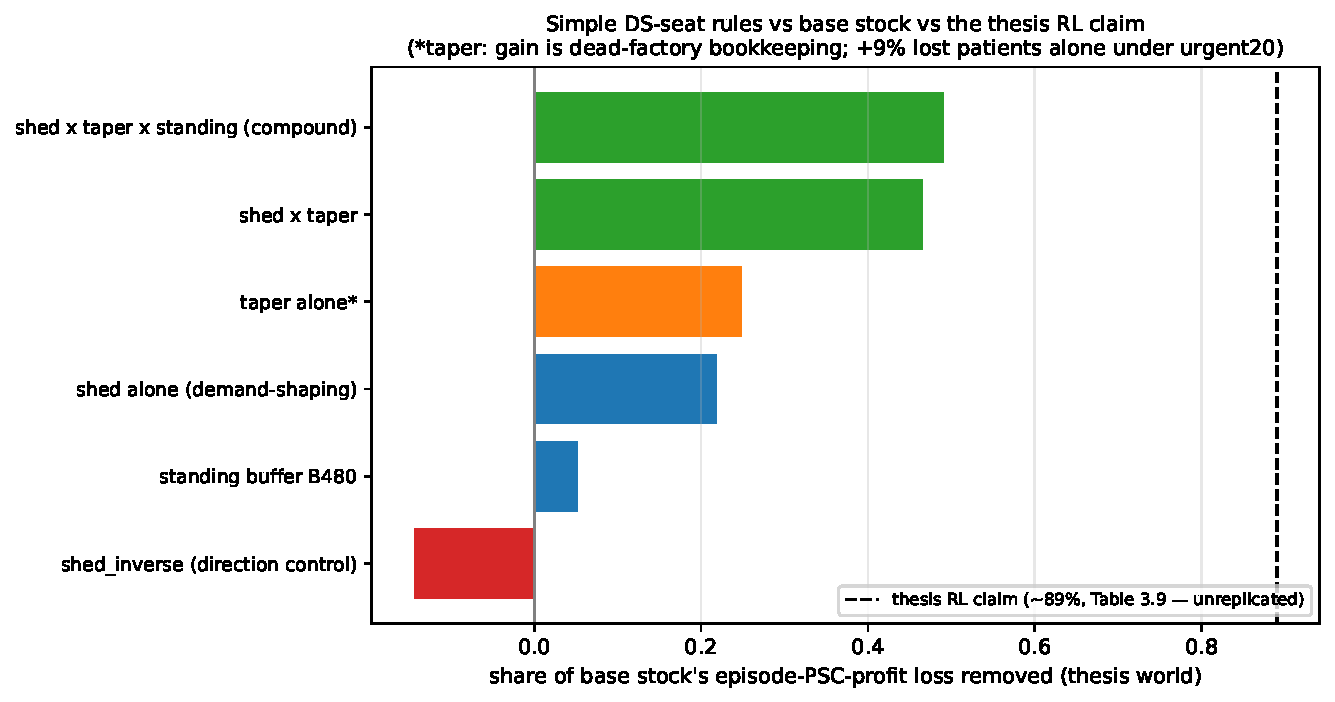
\includegraphics[width=0.78\textwidth]{../value_decomposition_study/results/figures/ds_seat_shares.pdf}
\caption{F2 in one picture: simple distributor rules vs the RL claim, thesis world,
audited reporting seeds.}
\end{figure}

\textbf{F3 --- When supply is genuinely short, what matters is where reserve stock sits
and how big it is --- both computable in advance from observable quantities; reacting
cleverly during the outage does not help.}
The evidence: under scarcity the cost--service frontier is owned by a single
composition (buffer $+$ reroute $+$ taper); the buffer's optimal \emph{location} flips
to the disrupted chain once the surviving chain is too weak to carry the load; and
demand-aware \emph{sizing} --- buffer $=$ (demand $-$ surviving deliverable)
$\times$ duration --- cuts lost patients from 505 to 41.
\emph{Meaning: the two deployable decisions that matter are where stock sits and how it
is sized --- both computable from observables, no learning required.}

\textbf{F4 --- Every adaptive ``smart'' rule we tested made the system worse; simple
static structure won every time.}
The evidence: across three studies, every reactive rule backfired ---
delivery-rate detection, backlog-priority allocation, serve-the-captive (in the
routing-repaired world), rotating priority, priority-with-floor, and both severity-aware
redirect caps. The mechanism is structural: the trust feedback loop rewards consistency,
and the surviving manufacturer's production is driven by the orders it receives, so
clever order withholding starves the very supply it is trying to protect.
\emph{Meaning: for the eventual RL comparison, the honest prior is that adaptivity
must overcome a measured pattern of adaptive rules underperforming static structure.}

\begin{figure}[t]
\centering
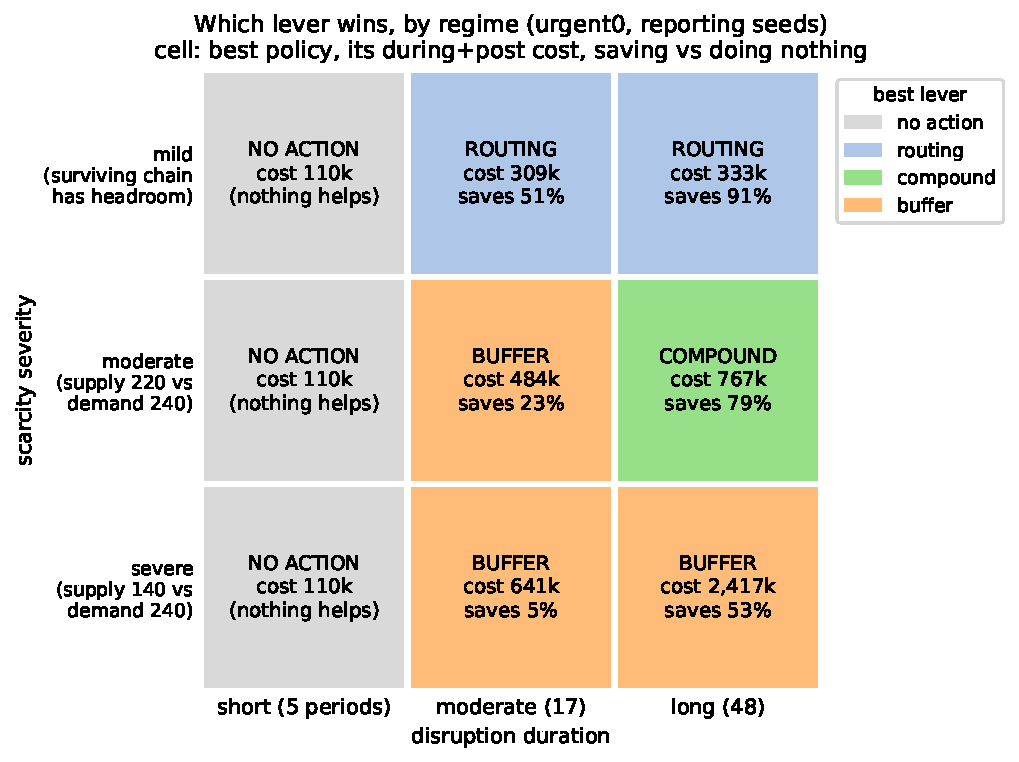
\includegraphics[width=0.7\textwidth]{../value_decomposition_study/results/figures/lever_flip_map.pdf}
\caption{F3 in one picture: the lever-flip map over the severity $\times$ duration plane.
Each cell's color indicates the winning lever (no-action $\to$ routing $\to$ compound
$\to$ buffer-only); the severe-scarcity cell is corrected to a disrupted-located buffer.
Cell color encodes WHICH lever wins; cell text gives that policy's cost and its saving
versus doing nothing. The recurring-disruption robustness check has since been run and
PASSED: with two events per episode no cell changes its winner, so the map stands.}
\end{figure}

\section{Phase-by-phase detail}\label{sec:detail}

\subsection{Background: the DRL arc (why there is no working RL comparator)}
The reward audit found reward components 1 and 4 carrying a thesis-level algebraic
defect, component 5 a code defect, and components 2/3/6 saturated as configured; repairs
un-stuck all six components. Training instability traced to the adaptive exploration
rule (a multiplicative update that runs away to its cap); a linear schedule yields a
stably-training agent --- which then \emph{loses} to base stock on system profit
($-$4.06M vs $-$2.35M, driven by manufacturer queue cost). The thesis's headline RL
result (its Table 3.9) is therefore treated as a claim, not a reproduced result, pending
the author's configuration.

\subsection{Routing study (thesis severity)}
The captive health center's hard-wired equal split, plus stranded-order suppression
(orders stuck in a dead supplier's queue are never re-issued), lock $\sim$2/3 of the
disruption cost into the routing layer: trust-split $-$26\%, sharpened trust $+$
stale-order write-off $-$67\% (fill 1.000), oracle onset reroute $-$91\%; lost patients
1,768 $\to$ 203. Found en route: the normal demand model hard-reseeds the global random
number generator (all historical multi-seed normal-demand results were a single demand
path) --- fixed in our runners, gate-guarded.

\subsection{Understanding study (routing-repaired world)}
Allocation bounded at $\le$12\% via the maximum over the enumerated rule family (static
priority; fairness cost $\pm$0.023 fill); all dynamic rules backfire through the trust
loop. The residual disruption cost in the routing-repaired world decomposes into 41\%
dead-factory queue bookkeeping (dual cost accounting was introduced for exactly this),
the $\sim$10-period redirection transient, and a write-off glut later removed as a side
effect of instant rerouting.

\subsection{Value decomposition, Phase 1 (slack regime)}
Info-sharing reroute $\equiv$ oracle (bit-identical, audited); explicit delivery-rate
detection worse than the built-in trust mechanism (stock-cover masking $\sim$0.9M);
deployable compound 273k. Verification rebuilt the oracle as a true superset and corrected
two claims: foresight is worth $\sim$54k with the buffer at the SURVIVING chain, and
slack-regime buffers are negative only at the disrupted location ($+$4--7\% at the
survivor).

\subsection{Value decomposition, Phase 2 (scarcity regimes)}
With the surviving manufacturer also cut (to 50\% / 30\%), routing still reduces cost
($-$26\%/$-$50\%) but cannot create product (lost patients $\sim$flat across the entire
ladder); the compound reaches $-$79\% at fill 0.99--1.00; static priority flips harmful
($+$23\%); the severity$\times$duration map has two boundaries (stock-cover duration;
surviving-chain headroom), with sharp rerouting the WORST measured policy at severe
scarcity.

\subsection{Distributor-seat study (thesis world) and Part C}
Full-grid ladder over the distributor's complete decision space (everything else is dead by
topology). Results in F2/F4 and the claims tables. Part C: demand-aware buffer sizing (the
robust knob), the severe-scarcity buffer-location correction, and the redirect-cap
refutation with its mechanism (orders are the surviving supplier's production signal).

\section{Superseded claims (do not cite)}\label{sec:superseded}
\begin{itemize}
\item The $-$468k / $-$654k value split --- measured on the broken routing layer; retracted.
\item ``Permanent insurance captures 42\%'' --- broken-routing artifact; in the
routing-repaired slack-regime world, disrupted-located buffers are zero-to-negative
(surviving-located: $+$4--7\%).
\item ``Foresight adds nothing beyond the shared signal'' --- artifact of a mis-located
ceiling buffer; corrected to $\sim$54k ($\sim$5\%).
\item ``Detection captures $\approx$0'' --- true only for detect-then-buffer; rerouting
responses carry most of the onset value, and the upstream-signal trigger captures it fully.
\item ``Allocation $\le$12\% is the whole channel'' --- specific to the routing-repaired
world; in the thesis world the demand-shaping channel is worth $+$21.8\% (shed) and the
compound 49\%.
\item ``Fill 1.000'' for the 960-unit-buffer scarcity compound --- display-rounding;
0.990 (the 1,440-unit buffer reaches 0.9999).
\item The frozen per-severity buffer grids --- replaced by demand-aware sizing.
\end{itemize}

\section{Rigor record (one paragraph)}
All experiments ran on a gated harness (bit-exact baseline reproduction on both library and
CLI paths, determinism, demand conservation, cross-seed variance), with pre-registered
tuning/reporting seed splits (1--10 / 11--30), dual cost accounting, and both fairness
baselines carried. Every phase was audited by an independent agent re-deriving headline
numbers from raw CSVs (12/12, 11/12 --- the exception a display-rounding over-claim,
corrected --- 16/16, 13/13, and 18/18 for the robustness checks). Three contaminated or
buggy batches were caught by gates or
diagnostics (CLI-default contamination; a bootstrap deadlock; both logged) and discarded
without contaminating conclusions. Simulator defects found and guarded: the normal demand
model's global RNG reseed, a dead trust-delta config constant, the silent discard of
orders $\le$1 unit, and the missing on-order timeout that produces stranded-pipeline
suppression.

\section{Next steps}
\begin{enumerate}
\item \textbf{Obtain the thesis Table 3.9 configuration (incl.\ the base-stock baseline)} ---
decides the interpretation of F2's 49\%-vs-89\% gap; everything else is measured.
\item \emph{(Done since the last draft:)} the recurring-disruption robustness check
PASSED --- the map's winners are unchanged and the compound amortizes best; coverage does
not collapse in normal times (gated rules pay $\approx$zero premium); the shed rule's
equity profile is characterized. The map can be published as-is.
\item Ramped-onset regime as the second paper (the one place detection could earn value).
\item When corrected DRL code arrives: evaluate against the regime-appropriate simple
compounds (thesis world: the distributor-seat compound; slack regime: 273k; moderate
scarcity: 767k--1,726k with demand-aware buffer sizing), same seeds, same gates, both
accounting conventions.
\item Distill the paper from this document: the three-lever value decomposition with the
lever-flip map, the distributor-seat result as the RL-relevant centerpiece.
\end{enumerate}

\end{document}
